%\documentclass[12pt,a4paper, bibliography=totoc, listof=numbered, footexclude]{scrartcl}
\documentclass[12pt,a4paper, bibliography=totoc, listof=numbered, footexclude, BCOR=8.25mm, twoside]{scrartcl}
\usepackage[utf8]{inputenc}		
\usepackage[T1]{fontenc}     % T1: Kodierung mit der Latex speichert, fontenc: Kodierung, wie er Tastatureingaben interpretiert beim Compilieren
\usepackage[british,UKenglish,USenglish,english,american]{babel}
\usepackage{amsmath}
\usepackage{amsfonts}
\usepackage{amssymb}
\usepackage{graphicx}                         
\usepackage{float}
\usepackage{epstopdf}
\usepackage{caption}
\captionsetup{font=small}
\usepackage{tocloft}
\usepackage{fancyhdr}
\pagestyle{fancy}
\usepackage[]{acronym}
\newcommand{\acrounit}[1]{
  \acroextra{\makebox[18mm][l]{\si[]{#1}}}}
  \usepackage{siunitx}
  \renewcommand*{\bflabel}[1]{{\textsf{#1}\hfill}}
  
\begin{document}
 \title{Information transmission n                   }
 \title{Propagation of synchonous spiking in neural networks}
 \section{Introduction}
 \section{Methods}
 \subsection{Leaky integrate and fire model}
 To model electric neural properties a conductance based leaky integrate and fire model was used:
 \begin{align}
 \tau_m\frac{dV}{dt}= (-V + E_m) + R_m (- I_{K^+} - I_{syn} + I_{noise})
 \end{align}
 
 
 If the membrane voltage $V$ reaches the threshold  $V_{thresh}$, $V$ is being resetted to the resting potential and a spike is counted. To model the decreased probabilty of another spike shortly after a previous one, an absolute refractory period was introduced, which deactivates incoming inputs from other neurons.\\
 Additonally, a relative refractory period was used, which describes the increase of the $K^+$ conductance after an action potential and the subsequent exponential decay:
  \begin{align}
  \frac{d g_K}{dt}=-\frac{g_K}{\tau_K} \\
  I_K=g_k(V-E_K)
  \end{align}
  Hereby, the $g_K$ conductance is manually increased after a postsnyaptic spike emerged.
  \begin{align}
   	g_K \rightarrow g_K + {\tilde{g}}_K
  \end{align}
  Background activity was modelled by an Ornstein-Uhlenbeck process (OUP), which is described by a stochastic differntial equation and 
   \begin{align}
   \  \frac{d I_{noise}}{dt}=\frac{{I_\mu}-I_{noise}}{\tau_{OUP}} {+ \sigma \eta}
   \end{align}
  Used values for the mentioned parameters are as follows:
   \begin{acronym}[LONGEST]
      % Allgemein:
      % Als Beispiele:
      \acro{Dt}[\ensuremath{\Delta t}]{ \ \ 0.1 ms \ \ \ \ \ \ \ \ \ \ Simulation time step }
	 \acro{restPot}[\ensuremath{E_K}]{ \acrounit{-77 mV} \ \ \  \ \ \ \ $K^+$ equilibiurm potential }
	 \acro{Vtresh}[\ensuremath{V_{tresh}}]{ \acrounit{-55 mV} \ \ \  \ \ \ \ Spiking threshold }		
     \acro{eqPot}[\ensuremath{E_m}]{ \acrounit{-70 mV} \ \ \  \ \ \ \ Membrane resting potential}
     \acro{gconducadd}[${\tilde{g}}_K$]{ \ \acrounit{5 nS}   \ \  \  \ \ Additive K-conductance} 
     \acro{MemRes}[$R_m$]{ \ \acrounit{10$^7$ \ohm}   \ \  \  \ \ Membrane resistance}
     \acro{tausyn}[\ensuremath{\tau_{syn} }]{ \ \ 0.335 ms \ \  \ \ \ \ \ Synaptic time constant }
     \ Membrane resistance}
     \acro{tauOUP}[\ensuremath{\tau_{OUP} }]{ \ \ 5 ms \ \ \ \ \ \  \   \ \ \ \ \ Noise time constant }
     \acro{sig}[\ensuremath{\sigma }]{ \ \ 10$^{-7}$ \ \ \  \ \ \ \ \ \ \ \ \ Standard deviatoin of noise current }
      \acro{Imu}[\ensuremath{I_{\mu}} ]{ \ \  0.886 pA \ \  \ \ \   \ Mean noise current  }
              
          
              % % %
               
  
     
      %$\dot{\vec{M}}$
    \end{acronym}
 
  
  \subsection{Implementation}
  The network is implemented using an object-oriented approach in Python 2.7.
  The two main classes are the model neuron and the model synapse. \\
  Every model neuron has its own timing which updates instantaneously the conductance, current and voltage values. Every neuron creates a list of synapses, which all have the same strength. Every neuron from the previous group is connected to all neurons of the successive group, resulting in a fully connected feed forward network. \\
  Background activity is introduced via a noise object, that computes Ornstein-Uhlenbeck-process-like current using the Euler-Maruyama method, for every neuron.
  
  

  
  \section{Resuneuronlts}
  
  
  \begin{figure}
  \centering
  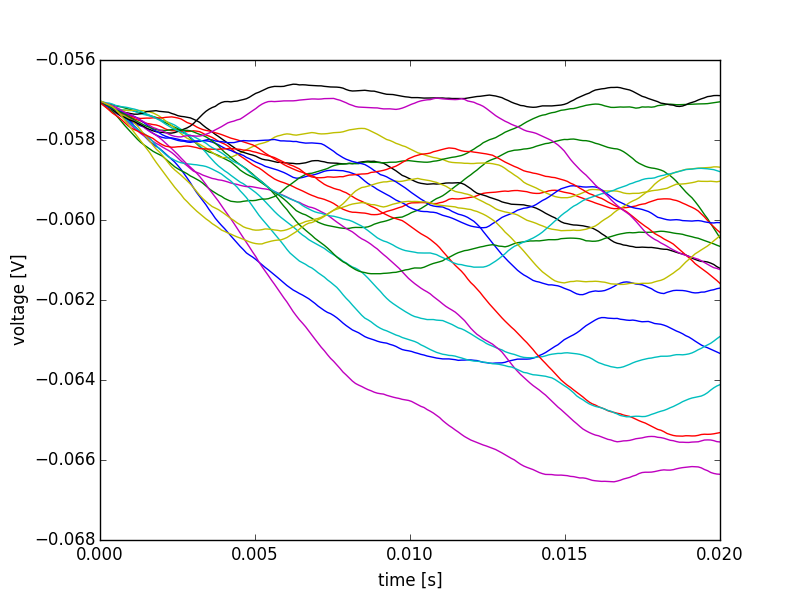
\includegraphics[width=0.7\linewidth]{./Plots/Our_Plots/noise}
  \caption{}
  \label{fig:noise}
  \end{figure}
  
  \begin{figure}
  \centering
  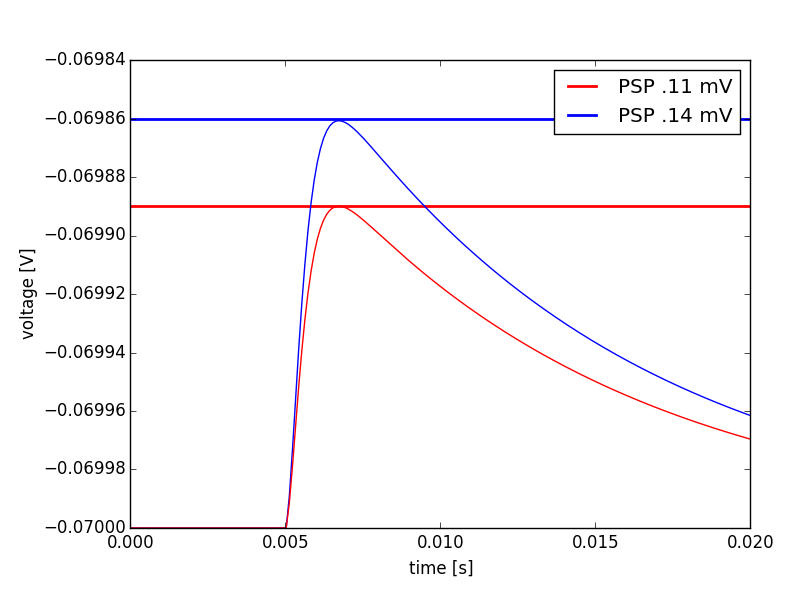
\includegraphics[width=0.7\linewidth]{./Plots/Our_Plots/PSP}
  \caption{}
  \label{fig:PSP}
  \end{figure}
  
  \begin{figure}
  \centering
  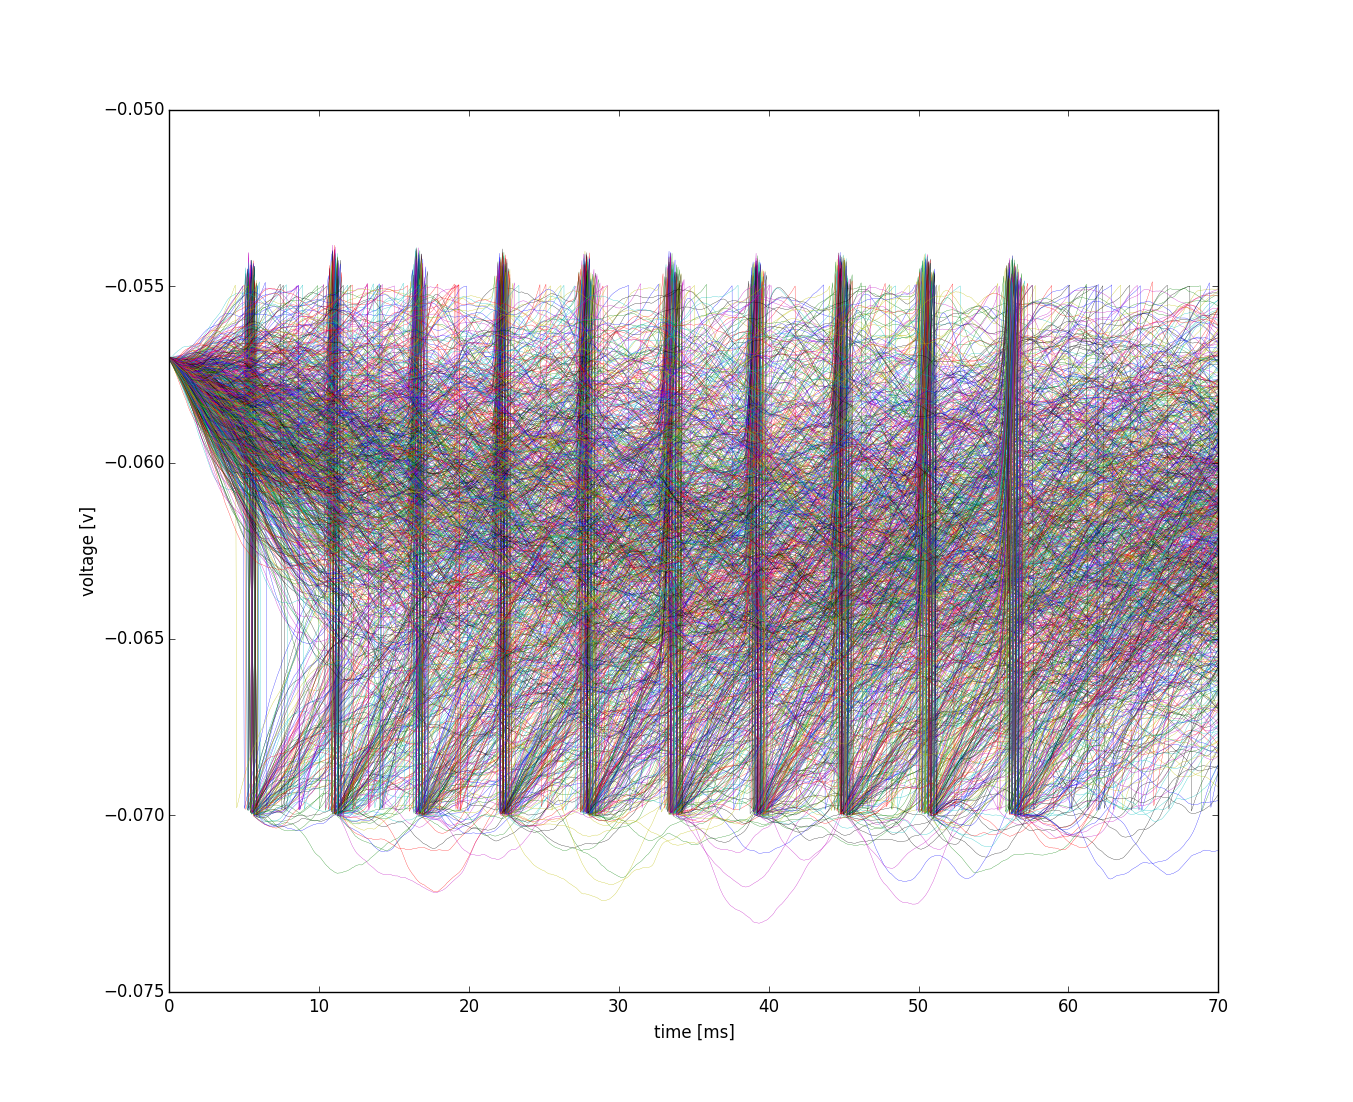
\includegraphics[width=1.0\linewidth]{./Plots/Our_Plots/voltageplot}
  \caption{}
  \label{fig:voltageplot}
  \end{figure}

  \begin{figure}
  \centering
  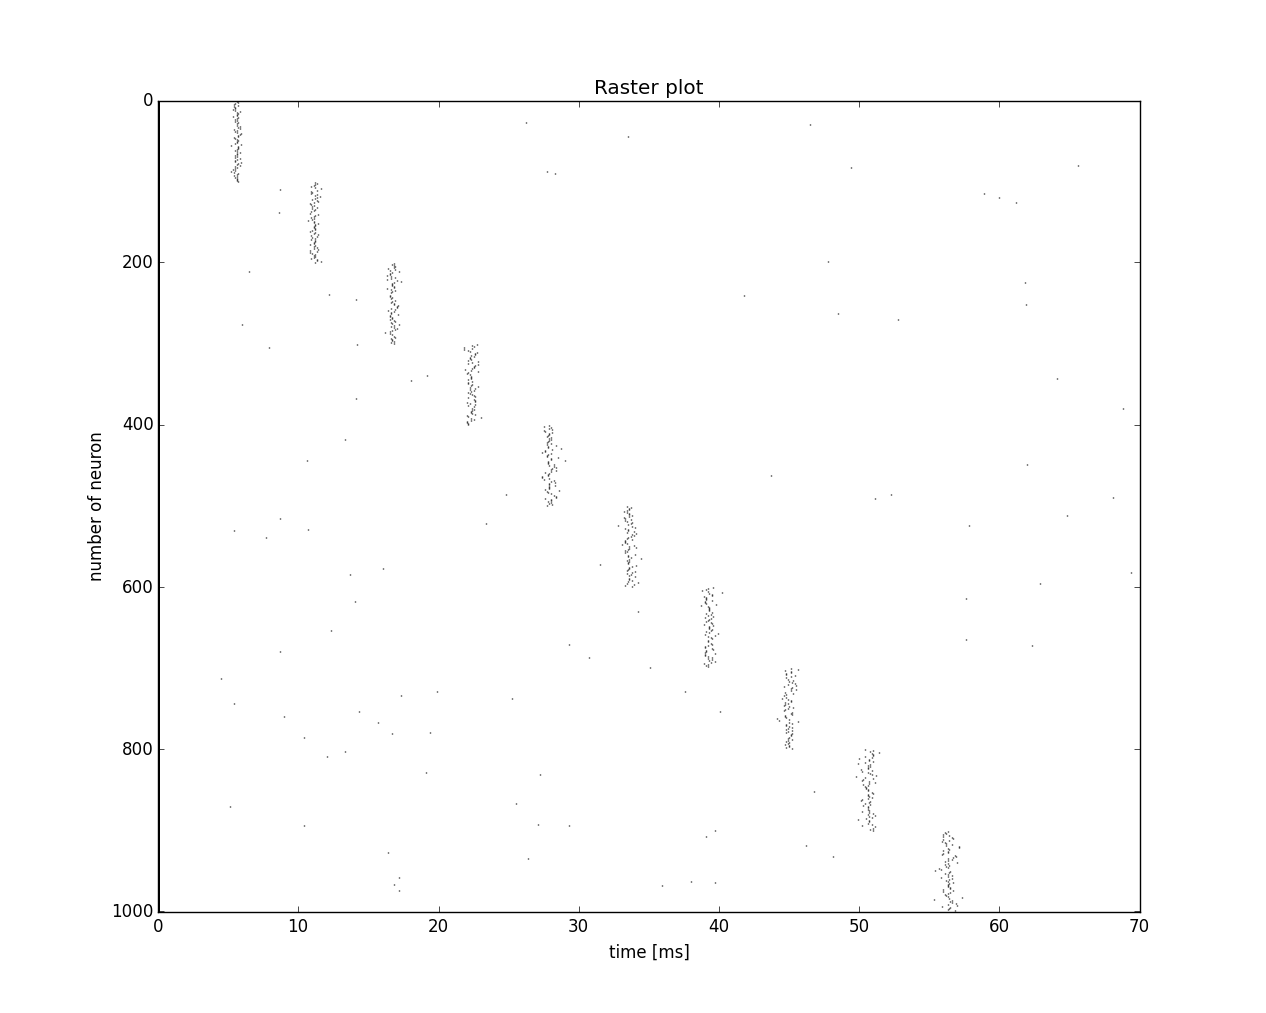
\includegraphics[width=0.7\linewidth]{./Plots/Our_Plots/rasterplot}
  \caption{}
  \label{fig:rasterplot}
  \end{figure}




  \section{Discussion}
 

\end{document}